\documentclass[a4paper,12pt]{article}

\usepackage[a4paper]{geometry}

\usepackage[utf8]{inputenc}            % Use utf8 input encoding
%\usepackage[latin1]{inputenc}         % Use iso 8859-1 encoding
\usepackage[T1]{fontenc}               % T1 fonts (support for accents/diacritics)
\usepackage{lmodern}                   % font with proper T1 support and good glyph quality

\usepackage{listings}                  % for (code) listings
\usepackage{amsmath}                   % AMS math typesetting
\usepackage{titlesec}

\usepackage{hyperref}                  % better references for PDF

\usepackage{graphicx}               % for graphics
\usepackage{algorithm}
\usepackage[noend]{algpseudocode}
\usepackage{siunitx}

\usepackage{pdfpages}

\titleformat{\section}{\LARGE\bfseries}% hide redundant number
            {}{0pt}{}
\lstset{language=Java}
\sisetup{locale = US}
\graphicspath{{pictures/assignment5/}}

\setlength{\parskip}{2ex plus0.5ex minus0.5ex}
\setlength{\parindent}{0em}

\begin{document}

\begin{center}
	\rule{\textwidth}{0.1pt}\\[1cm]
	
	\Large Softwarepraktikum SS 2019\\\bf Assignment 5
\end{center}

\begin{center}

	\rule{\textwidth}{0.1pt}\\[0.5cm]

	{\Large Group - 6\\[5mm]}

	\begin{tabular}{lll}

		Roman Vuskov & 376809 & roman.vuskov@rwth-aachen.de \\

		Songran Shi & 357791 & songran.shi@rwth-aachen.de \\

		Marlene Damm & 379945 & marlene.damm@rwth-aachen.de \\
		
		Marvin Gazibarić & 378154 & marvin.gazibaric@rwth-aachen.de \\

	\end{tabular}\\[0.5cm]

	\rule{\textwidth}{0.1pt}\\[1cm]

\end{center}

\newpage

\section{Task 1}
In our last assignment we implemented \texttt{IterationHeuristic} to give us a crude prediction of whether there is sufficient time for another search iteration. We hardcoded $0.2 \cdot T$ as the threshold beyond which no new search iteration shall be started, where $T$ is the total available time for the current move computation. This worked reasonably fine, especially for the specific setting of beam search with beam width 5.

Hence, we refined this heuristic to be more broadly applicable using statistical measures across many moves: During each move, we measure the actual elapsed time $t_n$ for each individual search iteration with depth $n$ and calculate the statistical mean $\mu_n$.

When it comes time to predict the time consumption for the next iteration with depth $n+1$ in a certain move, the average time consumption $\mu_n$ is compared to the time consumption $t_n$ of the last iteration, and we subsequently scale
the average time consumption $\mu_{n+1}$ of \emph{previous} moves accordingly to yield our prediction of $t_{n+1}$ in \emph{this} move:
\[t_{n+1} = \mu_{n+1} \cdot \frac{t_n}{\mu_n}.\]
This heuristic makes the intuitive assumption that the number of child nodes scales linearly with the number of parent nodes. We chose to base our prediction on the latest search iteration since it has the greatest search depth and thus provides the most information about an even deeper search.

Lastly, our \texttt{IterationHeuristic} includes two safety margins. One is fixed in size and is taken from the \texttt{PancakeWatchdog}. The other is relative to $T$, so that time panics are not triggered, if an estimation is just slightly wrong. A new search iteration is only given green light if the predicted time consumption falls below these thresholds:
\[t_{n+1} + \Delta t \leq (T -\SI{200}{\milli\s}) \cdot 0.9\,.\]
$\Delta t$ is the elapsed time until and including iteration $n$.

\newpage

\section{Task 2}

\subsection{Aspiration Windows}
Building upon the iterative deepening search algorithm from our last assignment, we have now extended our code to include Aspiration Windows. Conceptually, it is as simple as initializing each search tree node value with (one of) the aspiration window boundaries instead of $\pm \infty$. In practice, however, we need to be more cautious in the case of an empty window.

Let's assume that a certain Max-node has failed to find any move within the aspiration window. This node would then retain its initial value, which is the lower aspiration window boundary. Its parent node would then mistakenly include this empty node in its own evaluation. 

To prevent this, we have introduced a boolean node attribute \texttt{windowSuccess} to help discard these empty nodes. It is initialized as \texttt{false} and later set to \texttt{true} if a move is found in the aspiration window.

An exception to this is if the node in question has no legal moves at all. Since our method \texttt{getLegalMoves()} automatically reassigns \texttt{isMaxNode}, an empty return value indicates that the game phase has ended. This of course counts as a successful search. Furthermore, if we have reached the search depth of current iteration, we obviously need to assign window success to leaf nodes as well.

\subsection{Window Boundary Determination}
In each search iteration (except the first one) we center the aspiration window around the final root value of the previous search iteration, i.e. the value of the best move found so far. As for the heuristic for the window size, we save the values of all successful layer 1 nodes from the previous search iteration and calculate their standard deviation. 

The aspiration window boundaries are then $v \pm k \cdot \sigma$, where $v$ is the window center, $\sigma$ is the standard deviation and $k$ is a scaling factor the optimal value of which can be determined empirically.

\begin{algorithm}[H]
\caption{Aspiration window Node Evaluation}
\begin{algorithmic}
\Function{EvaluateNode}{$ $}
\Statex
\State \color{red} node value = aspiration window boundary 
\State node window success = false \color{black}
\Statex
\State legalMoves[move] $\gets$ \Call{GetLegalMoves}{$ $}
\Statex
\If{legalMoves is empty}
    \State \color{red} node window success = true \color{black}
    \State \textbf{return} value of current state
    
\Statex
\ElsIf{current layer == search depth}
    \State \color{red} node window success = true \color{black}
    \State \textbf{return} value of current state
\Statex
\ElsIf{this node is Max node}
    \For{\textbf{each} move in legalMoves}
        \State construct child node(current layer + 1, Min node, $\alpha$, $\beta$)
        \State \Call{EvaluateNode}{child node}
        \If{child node value > node value \color{red} \& child node window success \color{black}}
            \State node value = child node value
            \State \color{red} node window success = true \color{black}
            \State $\alpha$ = child node value
            \If{$\alpha \geq \beta$}
                \State break
            \EndIf
        \EndIf
    \EndFor
\Statex
\ElsIf{this node is Min node}
    \For{\textbf{each} move in legalMoves}
        \State construct child node(current layer + 1, Max node, $\alpha$, $\beta$)
        \State \Call{EvaluateNode}{child node}
        \If{child node value < node value \color{red} \& child node window success \color{black}}
            \State node value = child node value
            \State \color{red} node window success = true \color{black}
            \State $\beta$ = child node value
            \If{$\alpha \geq \beta$}
                \State break
            \EndIf
        \EndIf
    \EndFor
\EndIf
\EndFunction
\end{algorithmic}
\end{algorithm}

\newpage

\section{Task 3}
Frequent Aspiration Window Failures lead to a reduction in overall search depth and thereby weakening of the Ai. 

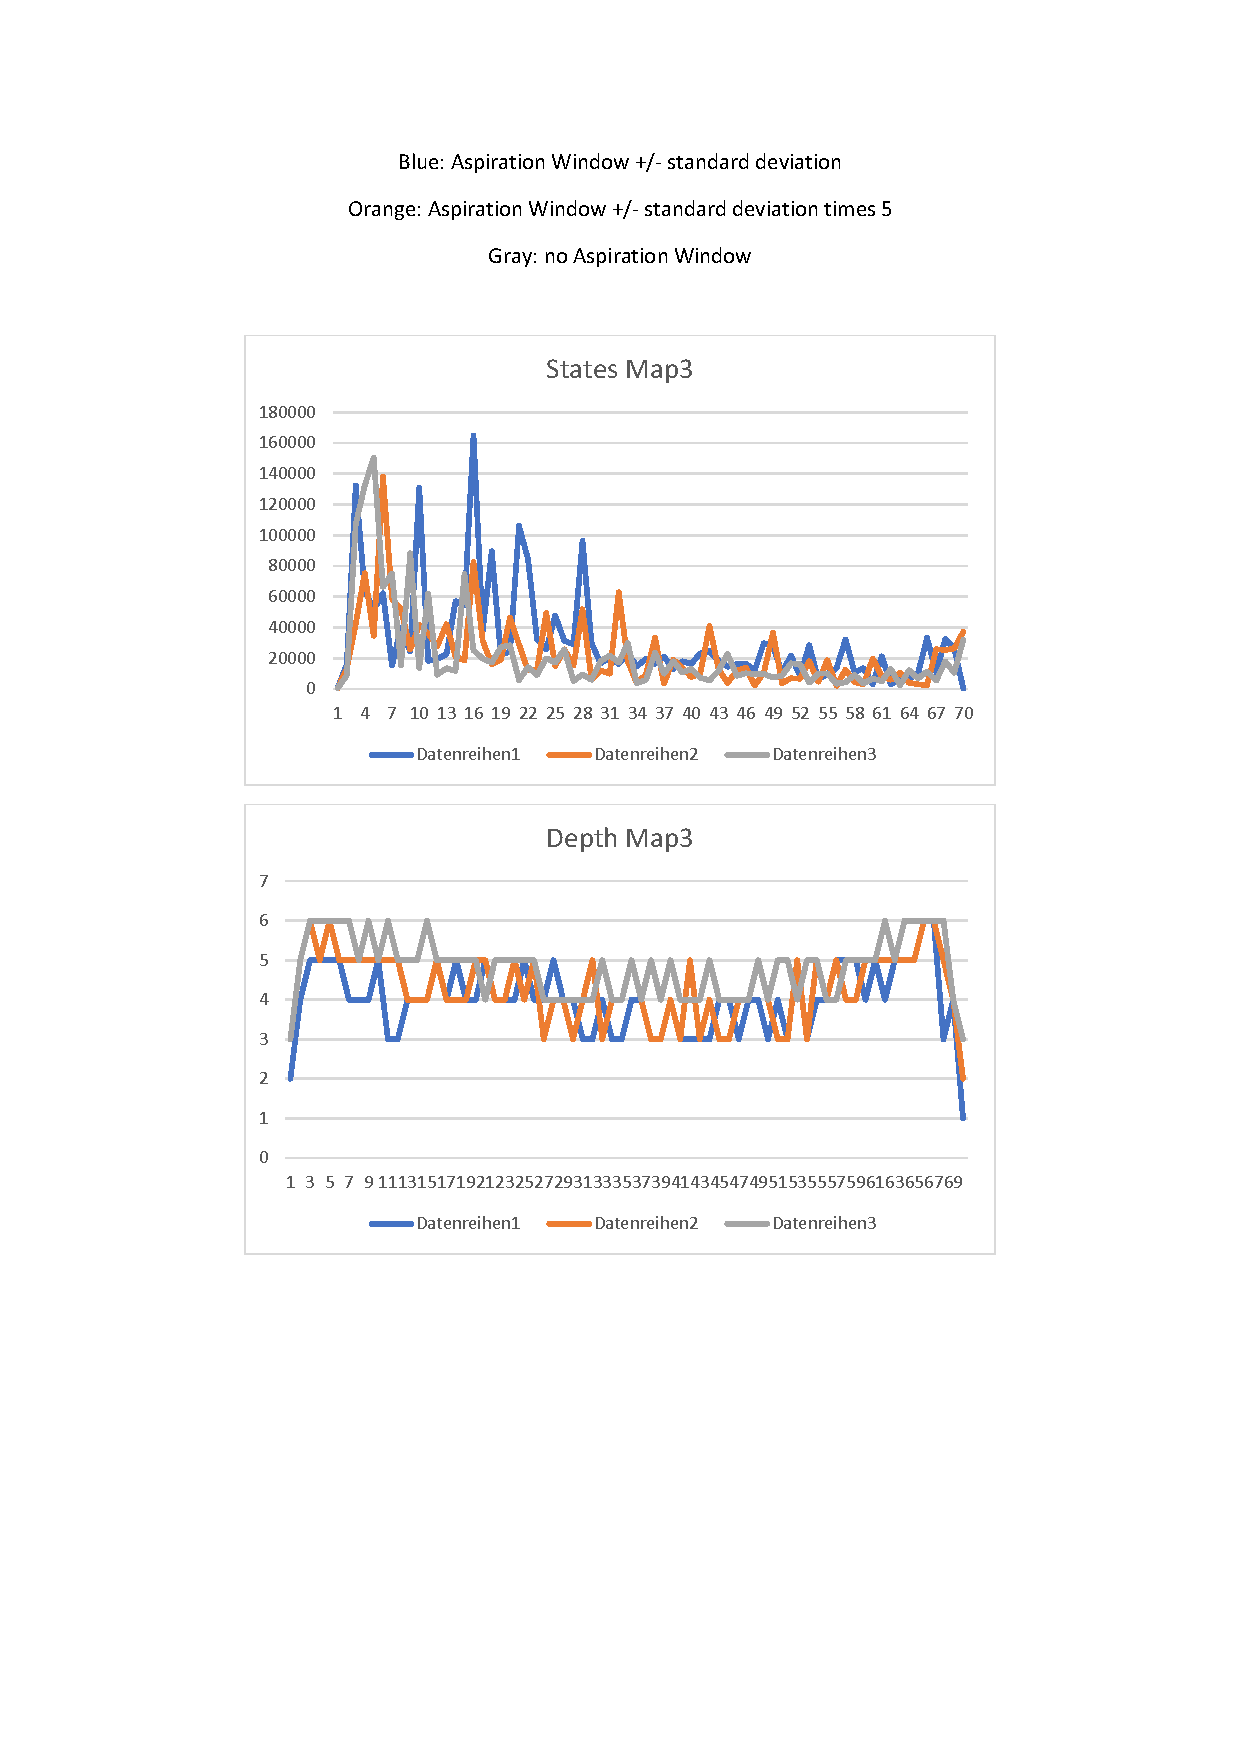
\includepdf[pages={1,2,3,4}]{exelPdf/asp.pdf}

\end{document}

